\documentclass[conference]{IEEEtran}
% \usepackage{cite}
\usepackage{tikz, pgfplots}
\usepackage{amsmath,amssymb,amsfonts}
% \usepackage{algorithmic}
\usepackage{graphicx}
\usepackage{multirow}
% \usepackage{textcomp}
% \usepackage{xcolor}
\pgfplotsset{compat=1.18}
\graphicspath{{./images/}}
\def\BibTeX{{\rm B\kern-.05em{\sc i\kern-.025em b}\kern-.08em
    T\kern-.1667em\lower.7ex\hbox{E}\kern-.125emX}}

\begin{document}

\title{Evaluation of the Parameterized-Response Differential Evolution Trader-Agent}

\author{\IEEEauthorblockN{George Herbert}
\IEEEauthorblockA{\textit{Department of Computer Science} \\
\textit{University of Bristol}\\
Bristol, United Kingdom \\
cj19328@bristol.ac.uk}
}

\maketitle

\begin{abstract}
This paper reports results from market experiments containing Paramaterized-Response Differential Evolution (PRDE) trader-agents.
Each PRDE trader-agent in a market simultaneously uses differential evolution (DE) to adapt their own trading strategy to maximise profitability.
The DE algorithm within each PRDE trader is governed by two parameters: the differential weight coefficient $F$ and the number in population $\mathrm{NP}$.
Markets containing a homogeneous population of PRDE traders exhibit different dynamics depending on the values of $F$ and $\mathrm{NP}$
The first part of this paper evaluates the effect that these two parameters have on the dynamics of the market; while the latter part of this paper proposes an extension to the PRDE algorithm to further maximise profitability.
\end{abstract}

\begin{IEEEkeywords}
Automated Trading, Financial Markets, Adaptive Trader-Agents, Differential Evolution
\end{IEEEkeywords}

\section{Introduction}

Adaptive automated trading algorithms have emerged as a transformative force in contemporary financial markets, enabling investors to harness the power of advanced computational techniques to gain a competitive edge in the marketplace.
Through the use of complex mathematical models and sophisticated algorithms, these cutting-edge technologies are able to analyse vast amounts of market data in real-time, identifying and exploiting trading opportunities with speed and accuracy that were previously unimaginable.
As a result, the use of adaptive automated trading algorithms has become increasingly prevalent, and has had a profound impact on the way in which financial markets operate, shaping the very fabric of the global economy.

However, the use of these algorithms has generated much discussion and debate among experts, with some cautioning against their potential drawbacks.
For example, the `flash crash' in US financial markets on 6 May 2010, which saw the Dow Jones Industrial Average plummet almost 1,000 points in a matter of minutes, has been attributed in part to high-frequency trading algorithms aggressively reselling short-term positions to one another.
Despite these concerns, it is clear these algorithms have become an inextricable part of the contemporary financial landscape, and their continued presence is all but guaranteed.
As such, researching these algorithms and their impact on contemporary markets is crucial for investors and researchers alike, in order to fully understand and navigate the rapidly evolving world of financial technology.

This report focuses on the \textit{Parameterized-Response Zero-Intelligence with Differential Evolution} (PRDE) trader-agent, which was recently introduced by Cliff in his research paper \cite{PRDE}.
The PRDE algorithm uses \textit{differential evolution} \cite{StornPrice} to continuously improve its trading strategy.
In his research, Cliff demonstrated that markets containing a homogeneous population of PRDE traders were overall more economically efficient than a baseline established when all traders were using a simple stochastic hill-climbing strategy optimiser.

However, the PRDE traders implemented in Cliff's experiments did not vary in their parameter values.
This present study builds on Cliff's research by exploring the effects of altering the two key parameters of the PRDE algorithm: the \textit{number in population} $\mathrm{NP}$ and the \textit{differential weight} $F$.
The $\mathrm{NP}$ parameter determines the number of strategies in a PRDE trader's private population, while the $F$ parameter determines the amount of perbutation applied to the strategies in the private population.

This present study examines the effects of changing these key parameters on market dynamics using the \textit{Bristol Stock Exchange} (BSE) (see \cite{BSE, BSEPaper}), an open-source, high-fidelity simulation of an LOB-based financial exchange.
By analysing the effects of changing $F$ and $\mathrm{NP}$ on the market behaviour, we can gain insights into how these algorithms influence market dynamics and how they can be optimized to maximize profitability.

\section{Background}

Gode and Sunder \cite{GodeSunder} revolutionised the field of experimental economics in 1993 with the advent of the \textit{Zero-Intelligence Constrained} (ZIC) trader-agent.
These agents, which simply generate quote prices uniformly at random from a predefined range, were shown to reproduce surprisingly human-like market dynamics.
In their original paper, Gode and Sunder defined the feasible range of trading prices as $[1,  200]$.
As such, a buyer with a limit price of $\lambda_B$ would generate quote prices from $\mathcal{U}(1, \lambda_B)$, whilst a seller with a limit price of $\lambda_S$ would generate quote prices from $\mathcal{U}(\lambda_S, 200)$.
Modern implementations of the ZIC model do not rely on a priori information about the feasible range, instead utilising the lowest and highest values in the order book as the bounds.
Cliff critiqued much of Gode and Sunder's work on ZIC in \cite{ZIP}, but nonetheless the ZIC model has become a widely used tool in the study of market dynamics.
Many subsequent \textit{zero-intelligence} (ZI) and \textit{minimal-intelligence} (MI) trader-agents have stemmed from the work of Gode and Sunder.

One such ZI trader-agent, \textit{Parameterized-Response Zero-Intelligence} (PRZI) \cite{PRZI}, was recently introduced by Cliff.
PRZI is a nonadaptive generalisation of ZIC, in which the shape of the probability mass function (PMF) used to generate quote prices is governed by a strategy parameter $s\in[-1, 1]\in\mathbb{R}$.
This $s$-value determines the degree of `urgency' or `relaxation' in the trader's behaviour.
As $s\to1$ the distribution is evermore biased towards `urgent' quote prices---those closest to the least profitable price for the trader, but most likely to attract a willing counterparty---conversely, as $s\to-1$, the distribution is biased towards `relaxed' quote prices---those that generate the most profit for the trader, but are considerably less likely to attract a counterparty.
When $s=0$, the PMF is uniform, identical to that of a ZIC trader.

\textit{PRZI with Stochastic Hill-Climbing} (PRSH) \cite{PRSH} is an adaptive extension to PRZI also introduced by Cliff.
The strategy parameter $s$ is dynamically altered by the algorithm in an attempt to increase profitability.
A given PRSH trader $i$ maintains a private local population $\mathcal{S}_i$ of $k$ strategy parameters; each of which it evaluates in turn via a loop to identify which is most profitable.
The most profitable strategy is `mutated' via a stochastic mutation function to produce $k-1$ mutants, and this set of $k$ strategies constitute the new $\mathcal{S}_i$.

\textit{PRZI with Differential Evolution} (PRDE) \cite{PRDE} is the latest adaptive extension to PRZI introduced by Cliff.
It replaces the simple stochastic hill-climber in PRSH with a DE optimisation system \cite{StornPrice}.
A given PRDE trader $i$ maintains its own DE system with a population of candidate $s$-values $\mathcal{S}_i$ of size $\mathrm{NP}\ge4$, which can be denoted by $s_{i,1},s_{i,2},...,s_{i,\mathrm{NP}}$.
Once trader $i$ has evaluated a particular strategy $s_{i,x}$, three other distinct $s$-value are chosen at random: $s_{i,r_1}$, $s_{i,r_2}$ and $s_{i,r_3}$ such that $x\ne r_1\ne r_2\ne r_3$.
A new candidate strategy $s_{i,y}$ is constructed as follows:
\[
s_{i,y}\leftarrow\max(\min(s_{i,r_1}+F_i(s_{i,r_2}-s_{i,r_3}),1), -1)
\]
where $F_i$ is trader $i$'s differential weight coefficient.
The fitness of $s_{i,y}$ is evaluated and if it performs better than $s_{i,x}$ then $s_{i,y}$ replaces $s_{i,x}$; otherwise, it is discarded and the next randomly selected strategy is evaluated.
PRDE also includes a `mega-mutation' mechanism to deal with convergence issues that arise from $s_{i,r_2}-s_{i,r_3}$ tending very close to zero in a highly-converged population.
If at any time the standard deviation of the candidate $s$-values in trader $i$'s private population is less than $0.0001$, then a randomly selected candidate $s_{i,r}$ is provided a value drawn at random from $\mathcal{U}(-1,1)$.

\section{Homogeneous Exploration of $F$ and $\mathrm{NP}$}

\subsection{Overview of the Combined Effect of $F$ and $\mathrm{NP}$}

According to Cliff's research in \cite{PRDE}, using DE as the adaption mechanism for each trading entity in a market can double the profit extracted through traders' interactions, compared to using a stochastic hill-climber as the adaption mechanism.
However, Cliff only experimented with values of $F=0.8$ and $\mathrm{NP}=4$ for the PRDE traders in the simulations he ran.
As such, my initial experiments in this paper serve as follow-up: to analyse the combined effect that different values of $F$ and $\mathrm{NP}$ have on the profitability.
I designed a set of experiments with a similar setup as Cliff, in which BSE was used to simulate a financial market for a single abstract tradeable commodity.
In each market simulation, I implemented a homogeneous population of $N_T=30$ PRDE traders with an equal number of buyers $N_B$ and sellers $N_S$ (i.e. $N_B=N_S=15$).
The population in a given experiment was homogeneous with respect to the fact that all PRDE traders had the same differential weight $F$ and the same number in population $\mathrm{NP}$.
Each simulation had what economists refer to as perfect elasticity of supply and demand: all $N_B$ buyers were provided a limit price of $\lambda_B=\$140$ per unit, whilst all $N_S$ sellers were provided a limit price of $\lambda_S=\$60$ per unit.
This produced a market in which every active trader could, in theory, find a willing counterparty to trade with.
In the simulation, after two traders engaged in a trade, they were rendered inactive until their stock was replenished, which occurred approximately every five seconds.
I ran each experiment for 100 simulated days on an Apple MacBook Pro with the M1 Pro chip, which took approximately three hours running at 800x real-time.

Figure \ref{profit_grid} displays a heatmap showing the combined profit extracted from the market by the population of $N_B$ buyers and $N_S$ sellers.
Considering each experiment used an identical quantity of traders and identical limit prices, the theoretical maximum profit that could have been extracted from each experiment was also identical.
As such, the actual total profit extracted is indicative of market efficiency.
There is a clear association between the configuration of $F$ and $\mathrm{NP}$ and the efficiency of the market.
Namely, large values of $F$ combined with moderately large values of $\mathrm{NP}$ produce the most efficient market.
$F=2$ and $\mathrm{NP}=14$ produced the most efficient market; 3.75\% more profit was extracted than the $F=0.8$ and $\mathrm{NP}=4$ configuration that Cliff used \cite{PRDE}.
However, the cause of this association is not obvious from inspecting the raw values.

\begin{figure}[htbp]
    \centerline{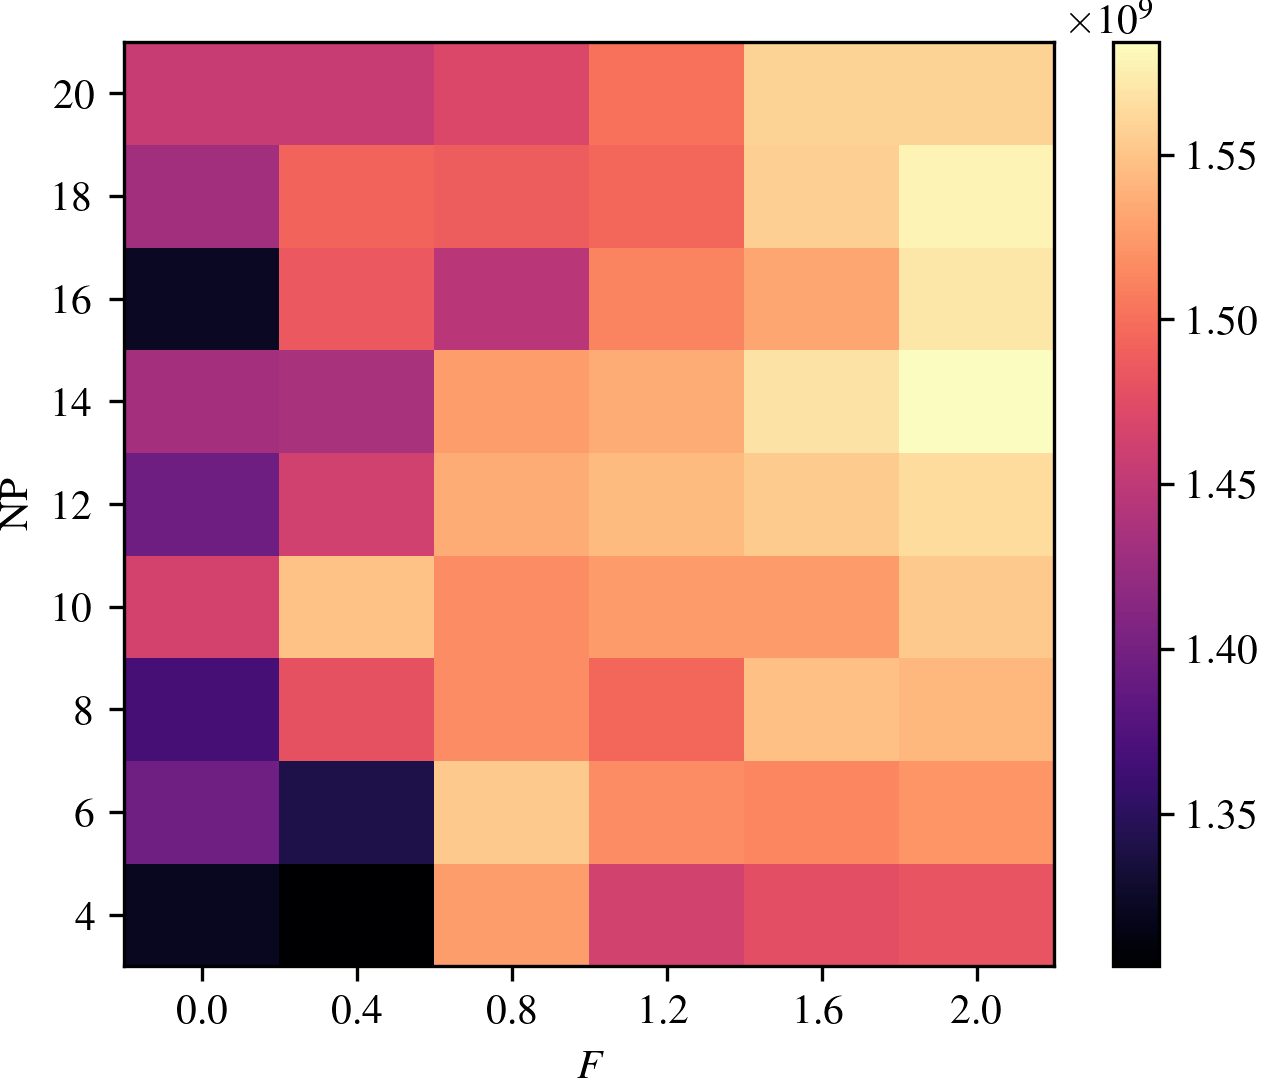
\includegraphics[width=\columnwidth]{profit_grid.png}}
    \caption{
        Relationship between different combinations of $F$ and $\mathrm{NP}$, and the total profit extracted by all PRDE traders in the market.
        Horizontal axis is $F$; vertical axis is $\mathrm{NP}$.
        The intensity of pixel shading represents the total profit extracted from the market during a single 100-day simulation.
        See text for further discussion.
    }
    \label{profit_grid}
\end{figure}

Much of the relationship can be attributed to the influence $F$ and $\mathrm{NP}$ have on the `urgency' of the traders in the market.
This is because there is a moderately strong positive correlation with $R^2=0.72$ between the total amount of time the traders in the market spent playing `very urgent' strategies (i.e. $s>0.5$) and the total profit extracted from the market, as evident in Figure \ref{strategy_profit}.

\begin{figure}[htbp]
    \centerline{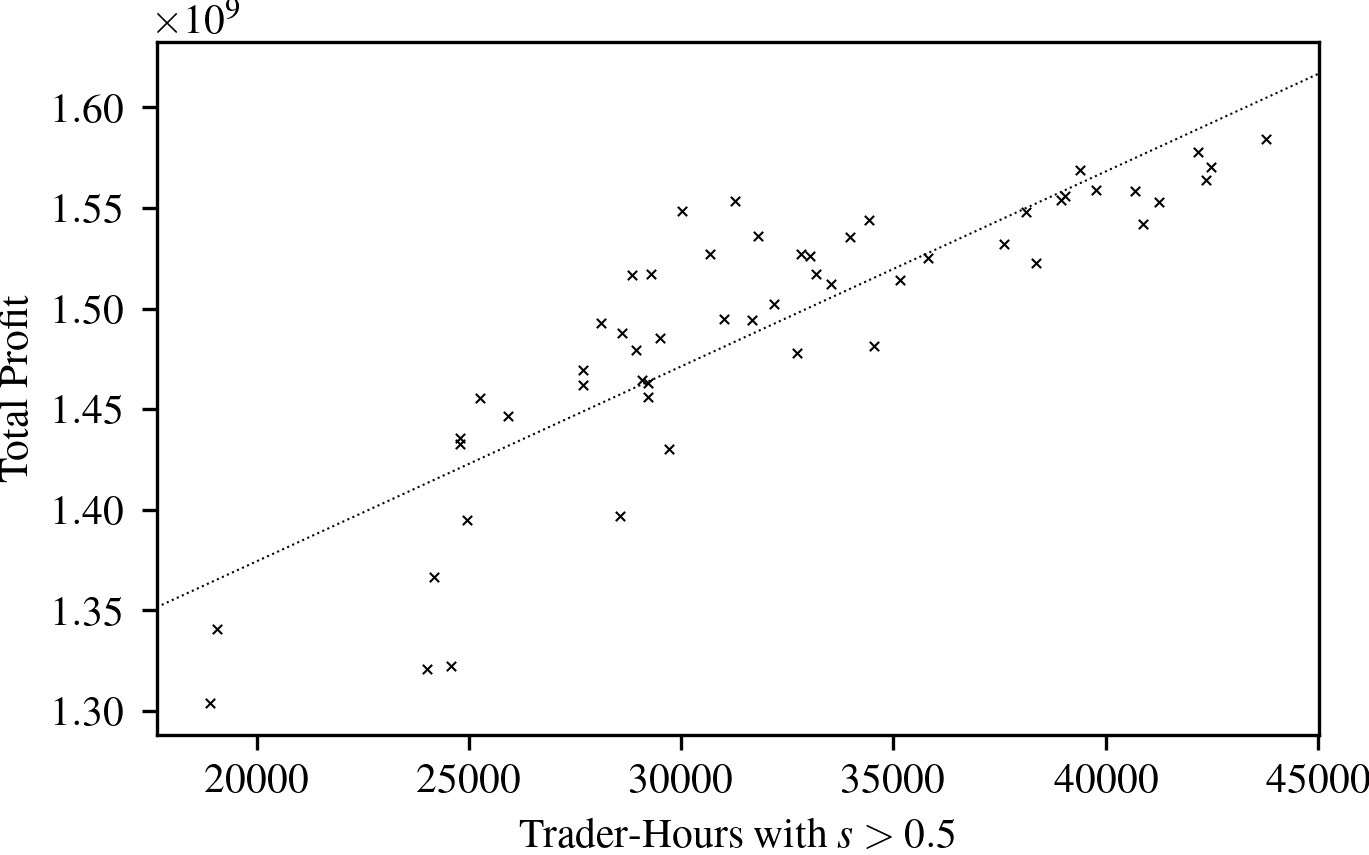
\includegraphics[width=\columnwidth]{strategy_profit.png}}
    \caption{
        Relationship between the amount of time traders spent playing $s$-values greater than 0.5 and the total profit extracted by all traders in the market.
        Horizontal axis is the number of trader-hours where $s>0.5$; vertical axis is the total profit extracted from the market during a given 100-day simulation.
        The line shows linear regression; $R^2=0.72$.
        See text for further discussion.
    }
    \label{strategy_profit}
\end{figure}

To understand this relationship, one must consider how the $s$-value of a given PRDE trader at a particular point in time affects the probability of it finding a counterparty to trade with.
For a given trader, as $s\to1$ (i.e. increasingly `urgent') the trader's quote prices are evermore likely to attract a counterparty; the reverse is true as $s\to-1$ (i.e. increasingly `relaxed').
As such, there is a strong relationship between the amount of time the traders in the market are `urgent' and the quantity of trades in the market session.
Due to each experiment having perfect elasticity of supply and demand, for a given trade at price $P$, the seller's profit can be denoted $P-\lambda_S$, whilst the buyer's profit can be denoted $\lambda_B-P$.
Therfore, the combined profit is as follows:
\[
  (P-\lambda_S) + (\lambda_B-P)=\lambda_B-\lambda_S
\]
In other words, the profit extracted from the market from any given trade is constant.
As such, the total profit extracted from the entirety of a given 100-day market session is directly proportional to the number of trades, which, as mentioned, is related to the amount of time traders in the market are `urgent'.

\subsection{Analysis of the Effect of $F$}

As mentioned, much of the variance in the efficiency of the market can be explained by the amount of time the traders spend playing $s$-values greater than 0.5.
To this end, the influence that the differential weight has on the total profitability can be primarily attributed to how it influences the `urgency' of the traders.
The data from the market simulations showed that there was a moderately strong positive corrlation with $R^2=0.77$ between $F$ and the amount of time the traders spent playing $s$-values greater than 0.5; this can be seen in Figure \ref{F_strats}.

\begin{figure}[htbp]
    \centerline{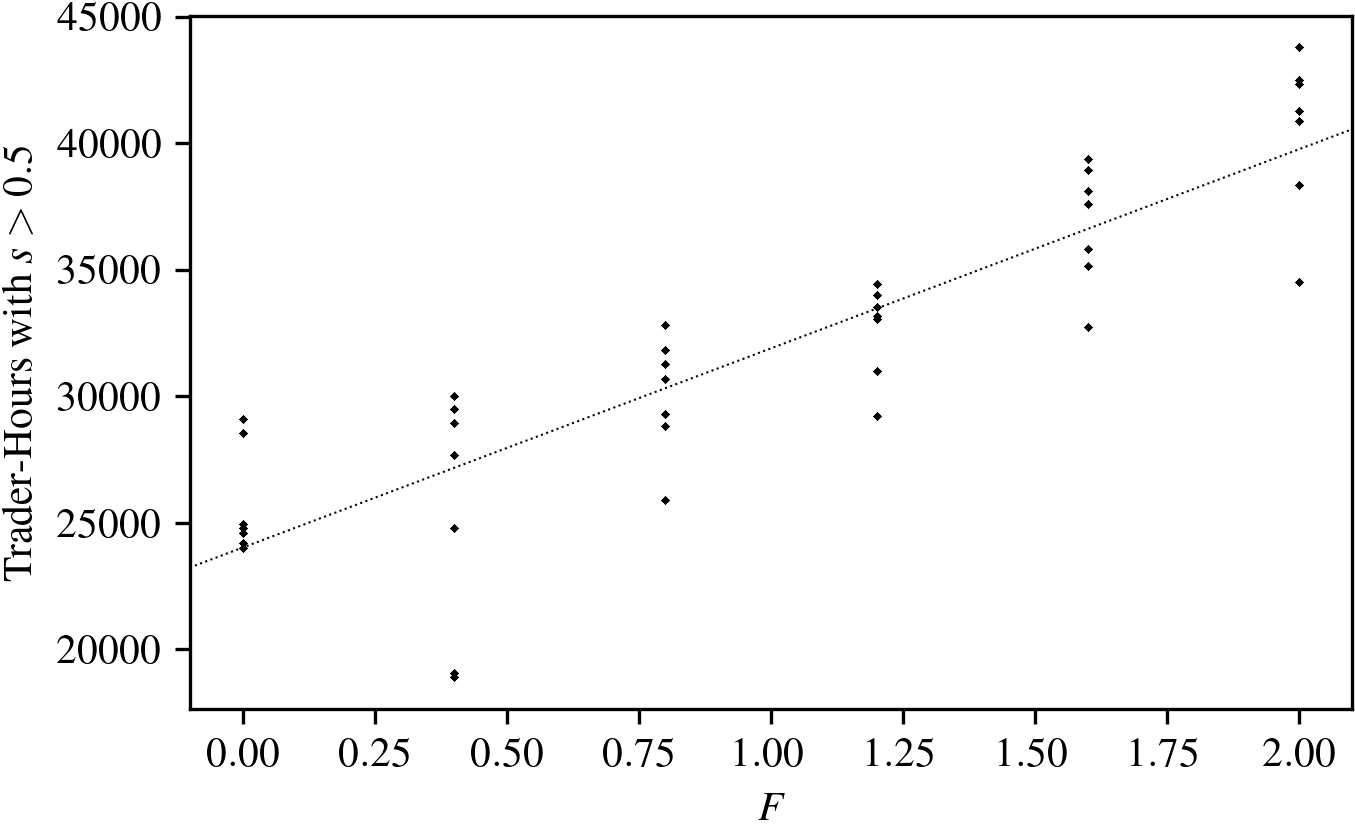
\includegraphics[width=\columnwidth]{F_strats.png}}
    \caption{
        Relationship between $F$ and the amount of time traders spent playing $s$-values greater than 0.5
        Horizontal axis is the differential weight coefficient $F$; vertical axis is the number of trader-hours where $s>0.5$.
        The line shows linear regression; $R^2=0.77$.
        See text for further discussion.
    }
    \label{F_strats}
\end{figure}

This relationship manifests due to the impact that $F$ has on the `urgency' of the PRDE traders throughout the entirety of the market session.
For larger values of $F$, the proportion of traders playing with $s>0.5$ increases significantly faster.
An example of this is shown in Figure \ref{k=14_strats} for when $\mathrm{NP}=14$.
When $F=2$, the proportion of traders trading with $s>0.5$ increased quickly: the seven-day moving average of the percentage of traders playing $s$-values that were $s>0.5$ rose to over 60\% after just 40 days.
Conversely, when $F=0.8$, the moving average was only approximately 45\% after the same amount of time.

\begin{figure}[htbp]
    \centerline{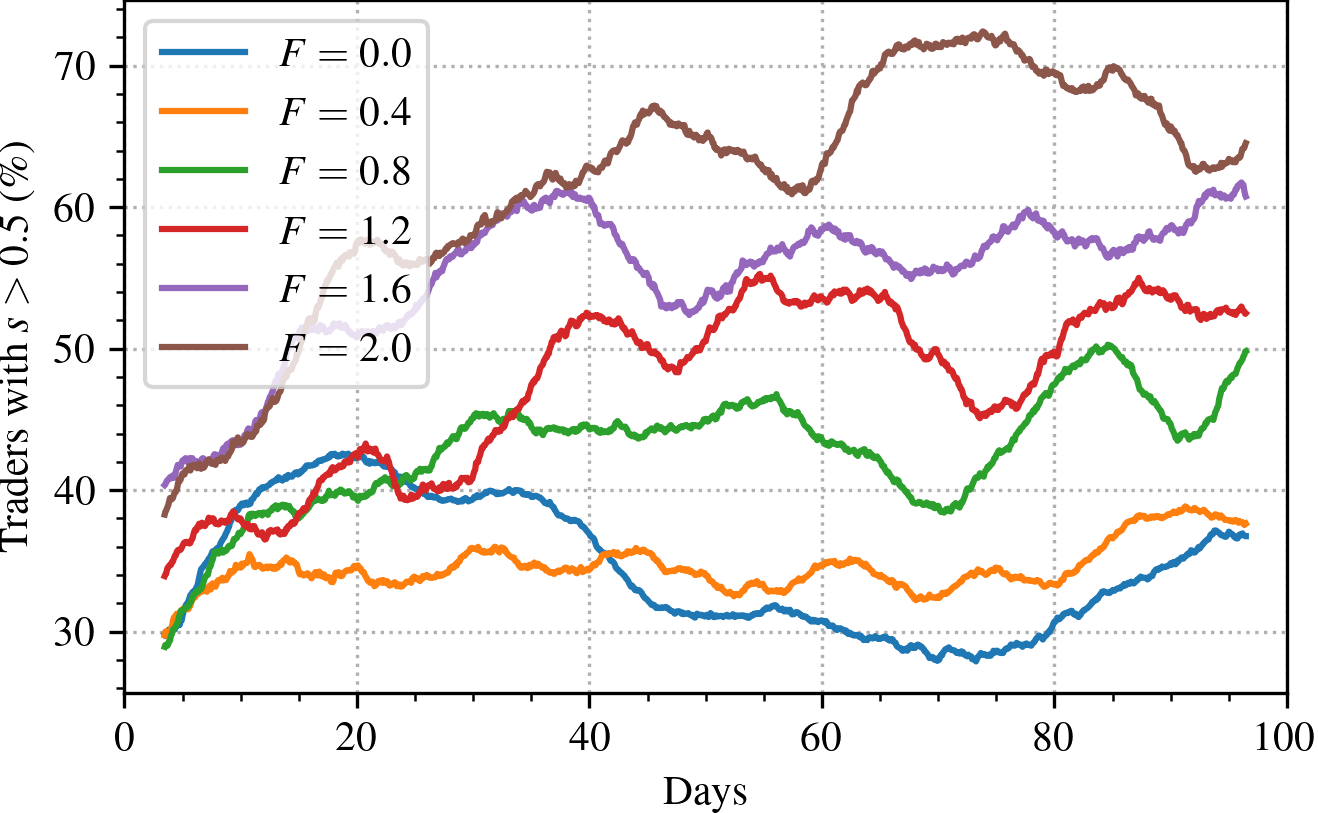
\includegraphics[width=\columnwidth]{k=14_strats.png}}
    \caption{
        Plot of the percentage of traders playing $s$-values of $s>0.5$ from multiple 100-day experiments in a market populated entirely by PRDE traders for different values of $F$ when $\mathrm{NP}=14$ 
        Horizontal axis is time, measured in days; vertical axis is the proportion of traders with an $s$-value of $s>0.5$.
        Each line is a seven-day simple moving average of the percentage for different values of $F$.
        See text for further discussion.
    }
    \label{k=14_strats}
\end{figure}

The reason for this effect can be explained mathematically.
Taking the extreme example of $F_i=0$ for trader $i$, the equation to derive a new candidate stratety $s_{i,y}$ to replace $s_{i,x}$ simply becomes $s_{i,y}\leftarrow s_{i,r_1}$.
Therefore, following the evaluation period of $s_{i,y}$, the value of $s_{i,x}$ can either remain the same, or take on the value of $s_{i,r_1}$, in which case two or more of the $s$-values in the local population $\mathcal{S}_i$ will be identical---the `genetic diversity' will be reduced.
In fact, the only time a new $s$-value can be introduced into $\mathcal{S}_i$ is when the diversity of $s$-values becomes so constrained a `mega-mutation' occurs, in which case a new $s$-value is sampled from $\mathcal{U}(-1,1)$.
As a result, the distribution of $s$-values in the entire population of PRDE traders struggles to deviate significantly from uniformity throughout the entirety of the 100-day market session.
This ultimately produces a market containing a wide range of both `urgent' and `relaxed' buyers and sellers, which is inefficient since many of the more `relaxed' traders will be unable to find a willing counterparty.
An example of such a distribution of $s$-values can be seen in Figure \ref{k=14,F=0.0_buy_strats}, which displays a heatmap of individual strategy values for the proportion of 15 PRDE buyers when $F=0$ and $\mathrm{NP}=14$.
While the case of $F=0$ is extreme, I found experimentally that the market increasingly exhibits the inefficient dynamics described here as $F$ tends towards $0$.

\begin{figure}[htbp]
    \centerline{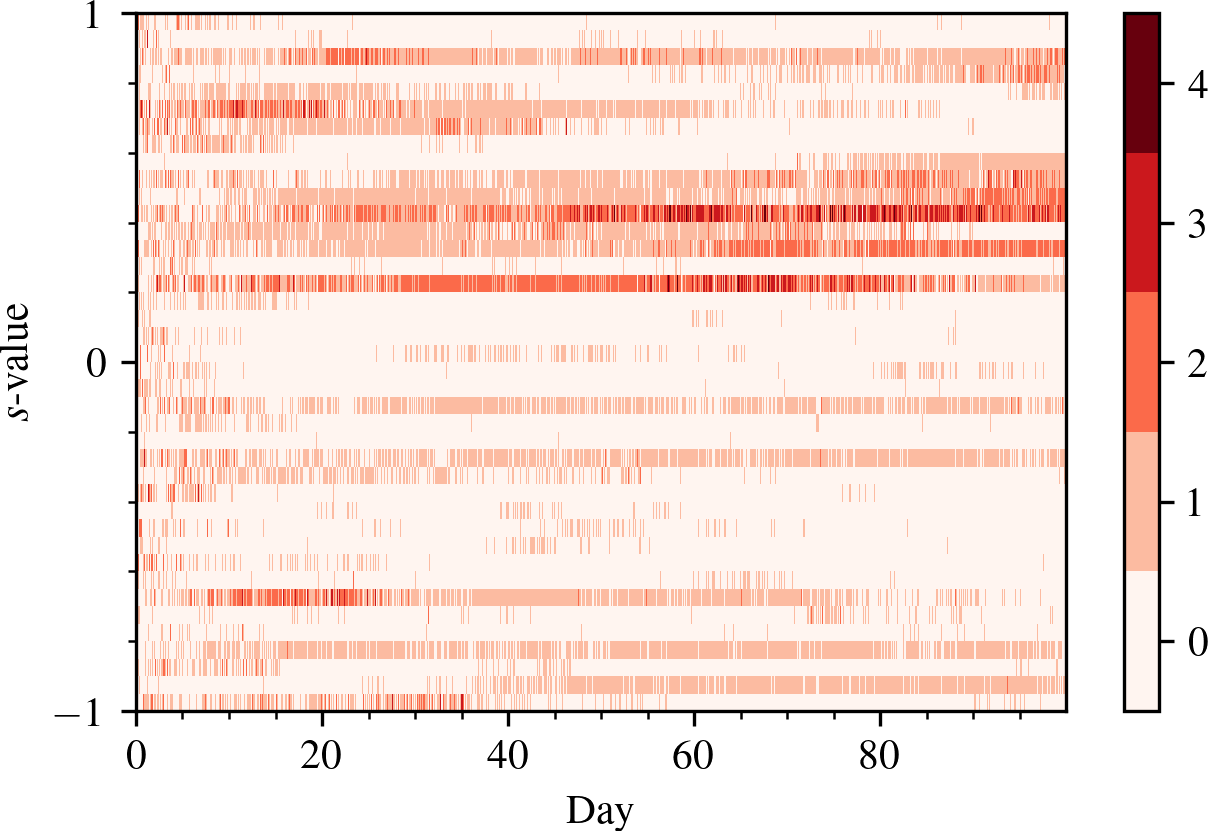
\includegraphics[width=\columnwidth]{k=14,F=0.0_buy_strats.png}}
    \caption{
        Heatmap of individual $s$-values for the population of 15 PRDE buyers in a market populated entirely by PRDE traders with $F=0$ and $\mathrm{NP}=14$.
        Horizontal axis is time, measured in days; vertial axis is the $s$-value pixelated into 40 bins of size 0.05.
        The intensity of pixel shading increases with the number of PRDE buyers in the population currently trading with an $s$-value in the 0.05 range.
        See text for further discussion.
    }
    \label{k=14,F=0.0_buy_strats}
\end{figure}

On the other extreme of the spectrum when $F=2$, a very different market dynamic tends to manifest.
This is evident in Figure \ref{k=14,F=2.0_buy_strats}, which displays a heatmap for the 15 PRDE buyers whereby $F=2$ and $\mathrm{NP}=14$.
Unlike the more uniform distribution of $s$-values exhibited when $F=0$, the $s$-values in Figure \ref{k=14,F=2.0_buy_strats} were bimodal at the two extremes of $s\approx-1$ and $s\approx1$, with the peak at $s=1$ being slightly larger.
Moreso, both the buyers and sellers displayed this behaviour.
Again, this can be explained mathematically using the equation to derive a new candidate stratety $s_{i,y}$ to replace $s_{i,x}$.
The value of the differential weight $F_i$ is directly proportional to $F_i(s_{i,r_2}-s_{i,r_3})$.
Thus, assuming $s_{i,r_2}-s_{i,r_3}$ is non-zero, the value of $s_{i,y}$ is more likely to be $-1$ or $1$ as $F_i$ increases.
This creates a market dynamic in which there is very quickly a number of of both extremely `urgent' and extremely `relaxed' buyers and sellers.
It is this large number of urgent traders that exist throughout the market session that enables a large amount of profit to be extracted from the market.
Furthermore, I found experimentally that for larger values of $F$, this bimodal behaviour is evermore prominant.

\begin{figure}[htbp]
    \centerline{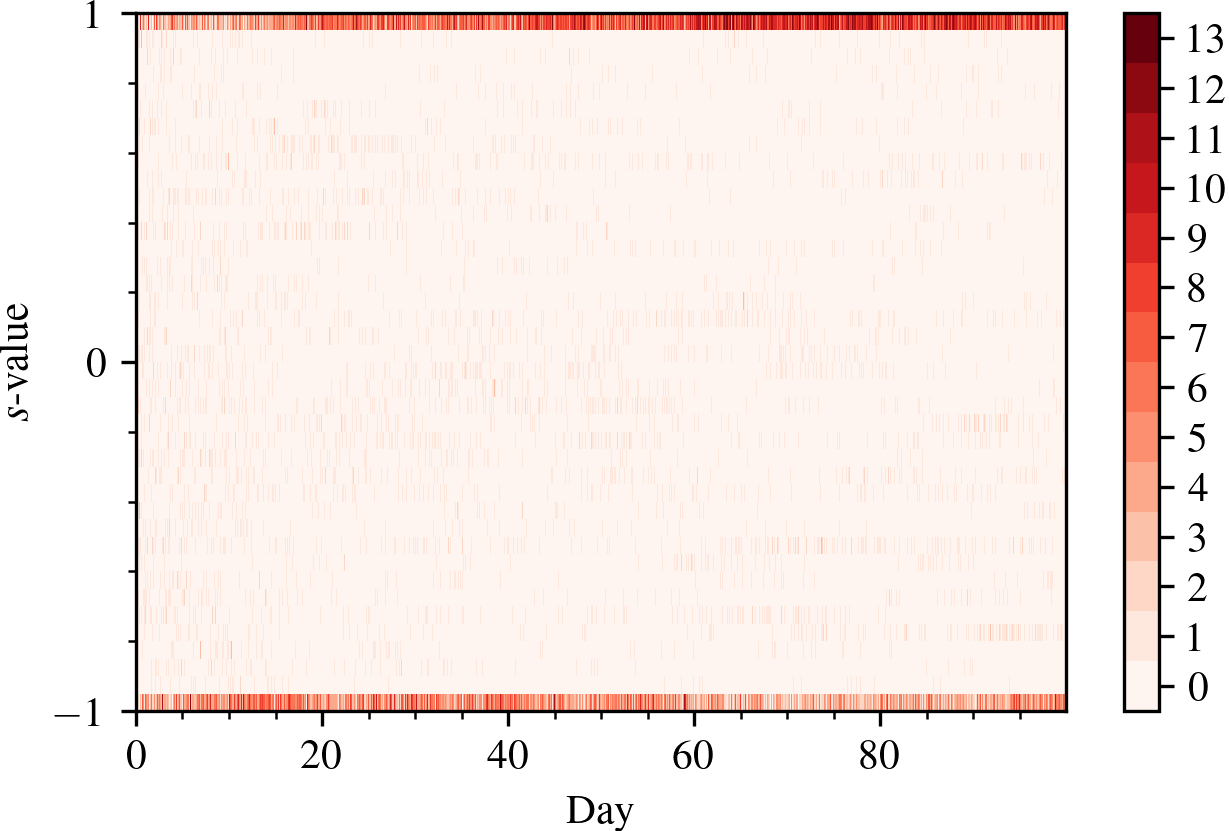
\includegraphics[width=\columnwidth]{k=14,F=2.0_buy_strats.png}}
    \caption{
        Heatmap of individual $s$-values for the population of 15 PRDE buyers in a market populated entirely by PRDE traders with $F=2$ and $\mathrm{NP}=14$.
        Format is the same as for Figure \ref{k=14,F=0.0_buy_strats}.
        See text for further discussion.
    }
    \label{k=14,F=2.0_buy_strats}
\end{figure}

\subsection{Analaysis of the Effect of $\mathrm{NP}$}

The effect of the number in population on the efficiency of the market is similar to that of the differential weight, in that it is primarily driven by its influence on the `urgency' of traders.
However, unlike the relationship with the differential weight, the relationship between $\mathrm{NP}$ and the amount of time traders spend playing $s$-values greater than 0.5 cannot be modelled linearly.
The data from the market simulations showed that the relationship is highly dependent on the value of $F$.
For smaller values of $F$, the influence of $\mathrm{NP}$ is significantly noisy, as shown in Figure \ref{profit_grid}.
However, for larger values of $F$, the relationship can best be modeled using a quadratic curve, as shown in Figure  \ref{F=2.0_strats}.
This indicates that the relationship between $\mathrm{NP}$ and the `urgency' of traders is more complex and dynamic than a simple linear model can capture.

\begin{figure}[htbp]
    \centerline{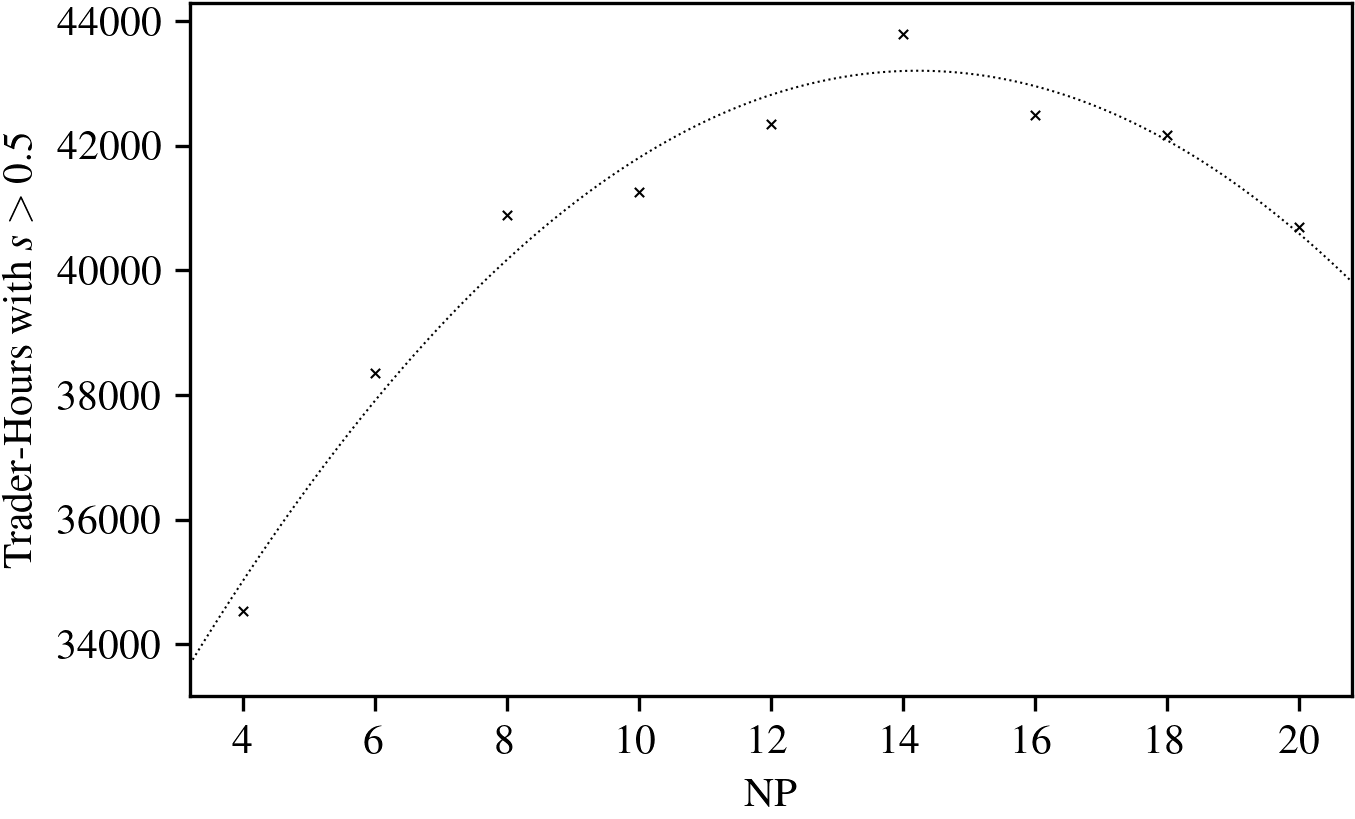
\includegraphics[width=\columnwidth]{f=2.0_strats.png}}
    \caption{
        Relationship between $\mathrm{NP}$ and the number of trader-hours in the market playing `very urgent' $s$ values greater than 0.5 when $F=2.0$.
        Horizontal axis is the number in population $\mathrm{NP}$; vertical axis is the number of trader-hours where $s>0.5$.
        The line shows quadratic regression; $R^2=0.96$.
        See text for further discussion.
    }
    \label{F=2.0_strats}
\end{figure}

This quadratic relationship can be explained as the combined effect of two influencing factors.
The first influencing factor comes from the effect that $\mathrm{NP}$ has on the number of $s$-values greater than 0.5 that a given PRDE trader $i$ can sustain in its private population $\mathcal{S}_i$.
The second influencing factor comes from the effect that $\mathrm{NP}$ has on the time it takes the traders in the market to improve on the initial random conditions.

As mentioned, larger values of $F$ induce a bimodal distribution of $s$-values at $s\approx -1$ and $s\approx 1$.
Using $\mathrm{NP}=\mathrm{4}$ as an example, an individual trader can have at most three $s$-values of $s\approx 1$, because as soon as the fourth $s$-value becomes 1, a `mega-mutation' occurs.
This equates to 75\% of the $s$-values in their private population $\mathcal{S}_i$ at $s\equiv 1$.
Conversely, when $\mathrm{NP}$ is larger, individual traders are able to accumulate a larger proportion of $s$-values of $s\approx 1$ in their private populations without a `mega-mutation' occurring.
This means that homogeneous populations of PRDE traders with larger values of $\mathrm{NP}$ produce a market dynamic with more `very urgent' traders, which produces a more efficient market.
This is also the reason that the effect of $\mathrm{NP}$ is more noisy for smaller values of $F$.
As mentioned, the bimodal distribution is everless prevalent with smaller values of $F$, so the impact of $\mathrm{NP}$ is less relevent as the `mega-mutations' do not occur as often.

The primary reason this trend is nonlinear because for especially large values of $\mathrm{NP}$, an inverse relationship between $\mathrm{NP}$ and the number of `very urgent' traders in the market manifests.
This is because, for a given PRDE trader, the probability than an $s$-value in the trader's private population is selected to be evaluated next is $\mathrm{NP}^{-1}$.
Therefore, in homogeneous populations of PRDE traders with larger values of $\mathrm{NP}$, it takes significantly longer to iteratively improve on the initial random conditions in the entire local population of $s$-values.
As a result, it takes significantly longer for the PRDE traders to accumulate a large number of $s$-values greater than 0.5, and as such the market is less efficient.
On the extreme end of the spectrum, as $\mathrm{NP}\to\infty$, the PRDE traders in the market would be completely unable to improve on the initial random conditions of the market.

\section{Heterogeneous Exploration of $F$ and $\mathrm{NP}$}

The experiments conducted to this point all involved homogeneous populations of PRDE traders in a simplistic market with perfect elasticity of supply and demand.
The results clearly showed that the markets containing PRDE traders with large values of $F$ and moderately large values of $\mathrm{NP}$, such as $F=2$ and $\mathrm{NP}=14$, managed to extract the most profit from the market.
However, this was simply because these combinations of $F$ and $\mathrm{NP}$ influenced the DE algorithm to sustain more highly `urgent' $s$-values.
Contemporary real-world markets are not comprised of homogeneous populations of automated trading-agents; real-world markets contain a multitude of different trading algorithms, all using different adaptive algorithms to maximise profitability, as well as a number of human traders.
Thus, I sought to investigate whether the profitability of a given combination of $(F, \mathrm{NP})$ in a homogeneous market was correlated to the profitability of the same combination in a heterogeneous market.
To do so, I ran a follow-up experiment with a very similar setup to that described previously to control for extraneous variables.
I similarly used BSE to simulate a financial market with $N_T=30$ PRDE traders with an equal number of buyers $N_B$ and sellers $N_S$ (i.e. $N_B=N_S=15$).
I used a limit price of \$140 per unit for the $N_B$ buyers and \$60 per unit for the $N_S$ sellers, and ran the experiment for 100 simulated days.
In fact, the only difference was the fact that I populated the market with heterogeneous PRDE traders rather than homogeneous PRDE traders.
I supplied each of the $N_B$ buyers and $N_S$ sellers an $(F,\mathrm{NP})$ combination from the 15 elements in the following set:
\[
  \left\{ (F, \mathrm{NP}) \mid F\in\{0, 0.4, 0.8, 1.6, 2\} \land \mathrm{NP} \in \{4, 12, 20 \} \right\}
\]
such that each buyer had a corresponding seller with the same element, but no two buyers or sellers had the same combination.

The total profit extracted from the heterogeneous market---which is indicative of market efficiency---was comfortably within the range of the homogeneous experiments at approximately 1.43 billion.
In fact, it was within 1\% of the mean profit extracted from the homogeneous experiments in which the $(F,\mathrm{NP})$ combinations comprised the heterogeneous experiment.
% However, interestingly, there was no discernible relationship between the profitability of a trader with a given $(F, \mathrm{NP})$ combination in the homogeneous experiments and the same $(F, \mathrm{NP})$ in the heterogeneous experiment, as evident in Figure \ref{heterogeneous_homogeneous}.

\begin{figure}[htbp]
    \centerline{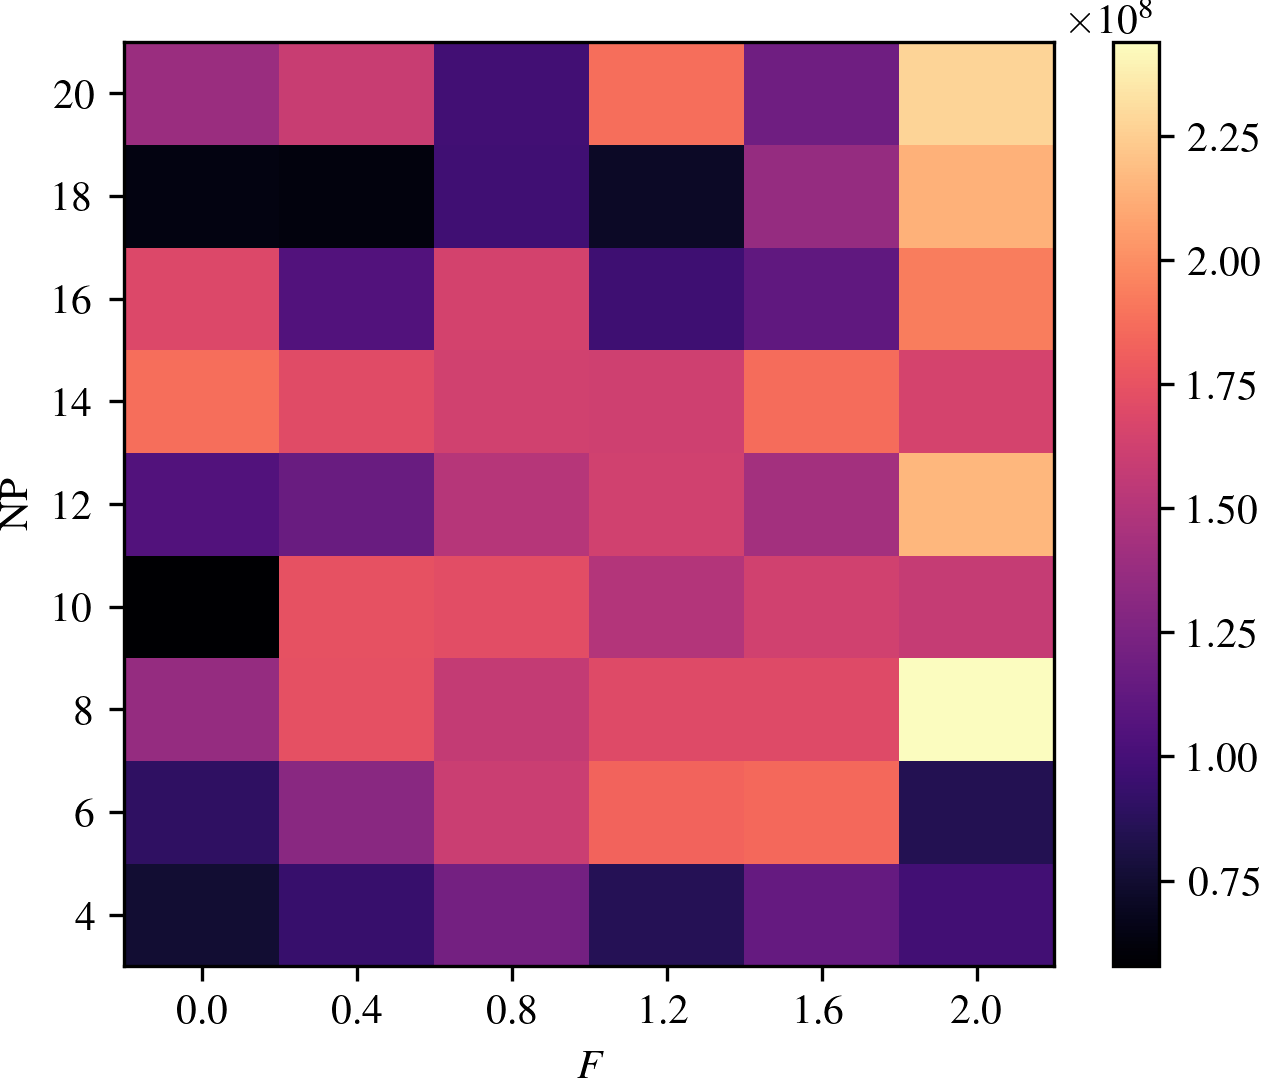
\includegraphics[width=\columnwidth]{zip_profit_grid.png}}
    \caption{
        Relationship between the differential weight coefficient $F$, the number in population $\mathrm{NP}$ and the total profit extracted by all PRDE traders in the market.
        Format is the same as for Figure \ref{profit_grid}.
        See text for further discussion.
    }
    \label{zip}
\end{figure}

\begin{figure}[htbp]
    \centerline{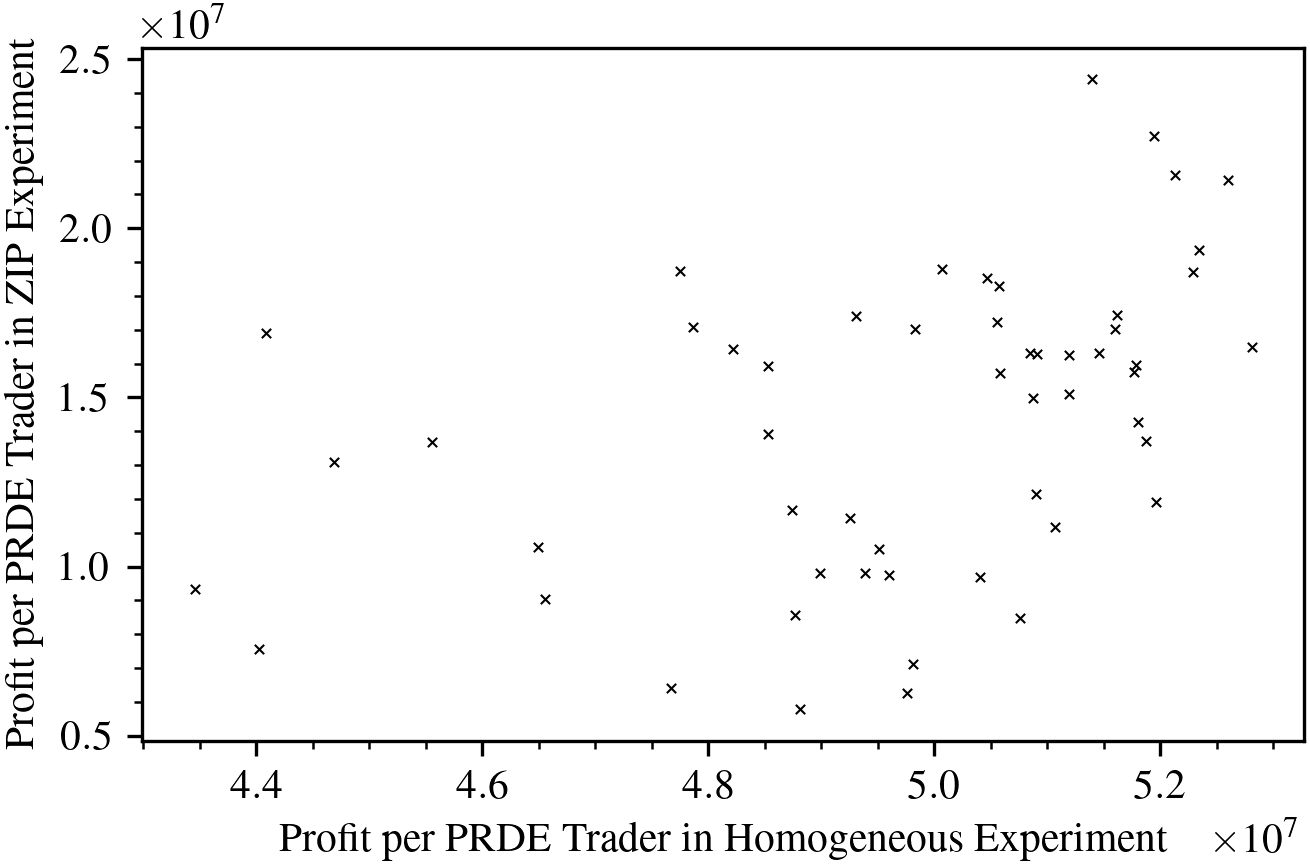
\includegraphics[width=\columnwidth]{homo_zip_scatter.png}}
    \caption{
        Relationship between the profitability per trader in the homogeneous PRDE experiments and the PRDE/ZIP experiments.
        Horizontal axis is the mean profit per trader in a given homogeneous experiment for a specific combination of $F$ and $\mathrm{NP}$; vertical axis is the mean profit per trader in a given PRDE/ZIP experiment for the same combination of $F$ and $\mathrm{NP}$.
        See text for further discussion.
    }
    \label{homo_zip_scatter}
\end{figure}

This indicates that the effect of $F$ and $\mathrm{NP}$ differs according to the population of traders in the market.
In effect, there is no absolute `optimal' combination that will consistently extract the maximum profit, because the behaviour of the other traders in the market strongly influences the control that $F$ and $\mathrm{NP}$ have.

\section{Extending PRDE}

\subsection{Motivation}

The experiments showed that the behaviour of the PRDE traders was highly influenced by the differential weight coefficient $F$ and the number in population $\mathrm{NP}$.
Moreso, it was evident that no one combination was consistently most profitable---the profitability was highly dependent on the other traders in the market, as well as the type of market.
As such, I hypothesised that a trader similar to PRDE, that automatically controlled the value of $F$ would be far more profitable across a variety of different markets.

\subsection{JADE}

JADE \cite{ZhangSanderson} is a DE algorithm that automatically updates the control parameter $F$ to appropriate values, and therefore removes the requirement for a user to have prior knowledge about the relationship between $F$ and the characteristics of the optimisation problem.
In light of this, I replaced the DE/rand/1 variant in PRDE with a variant of the JADE algorithm to produce a new trader agent: \textit{Parameterized-Response Zero-Intelligence with JADE} (PRJADE).
I hypothesised that PRJADE would provide better performance across a range of different markets, since the user would not require prior knowledge of the market dynamic.

To implement JADE in PRJADE, I implemented a variant of the DE/Current-to-$p$-best/1 with archive mutation strategy \cite{ZhangSanderson}.
Each PRJADE trader maintains its own JADE system with a population of candidate $s$-values of size $\mathrm{NP}\ge 4$, which for trader $i$ in generation $g$ can be denoted by 
\[
    P=\{s_{i,g,1}, s_{i,g,2},...,s_{i,g,\mathrm{NP}}\}
\]
Once a particular strategy $s_{i,g,x}$ has been evaluated, three other distinct $s$-values are chosen: $s^p_{i,g,\text{best}}$ is randomly chosen as one of the top $p\%$ individuals in the population $P$; $s_{i,g,r_1}$ is randomly chosen from the population $P$ such that $s_{i,g,r_1}\ne s^p_{i,g,\text{best}}$; and $\tilde{s}_{i,g,r_2}$ is randomly chosen from $P\cup A$ such that $\tilde{s}_{i,g,r_2}\ne s_{i,g,r_1}\ne s^p_{i,g,\text{best}}$.
$A$ is an `archive' set of $s$-values: those $s$-values that previously failed in the selection process.

The mutation $s$-value in PRJADE is computed as follows:
\[
    s_{i,g,y}=s_{i,g,x}+F_i\left(s^p_{i,g,\text{best}} - s_{i,g,x}\right) + F_i\left(s_{i,g,r_1} - \tilde{s}_{i,g,r_2}\right)
\]
The fitness of $s_{i,g,y}$ is evaluated and if it performs better than $s_{i,g,x}$ then $s_{i,g,y}$ replaces $s_{i,g,x}$ in generation $g+1$; otherwise, it is discarded and the next strategy in the sequence $s_{i,g,x+1}$ is evaluated.

\subsection{Results}

\section{Conclusion}

\bibliographystyle{IEEEtran}
\bibliography{refs}

\end{document}
